%%%%%%%%%%%%%%%%%%%%%%%%%%%%%%%%%%%%%%%%%%%%%%%%%%%%%%%%%%%%%%%%%
\chapter{YÖNTEM}\label{CH3}
%%%%%%%%%%%%%%%%%%%%%%%%%%%%%%%%%%%%%%%%%%%%%%%%%%%%%%%%%%%%%%%%%

Bu bölümde tehdit modeli, $\Pi_{\mathrm{ROI}}$ protokolünün yeniden üretimi, kullanılan veri kümeleri, iki saldırı, gerçekçilik testi, kök neden analizi ve savunmalar ile önerilen Odaklı Tam Şifreleme (FoveaHE) yöntemi ve değerlendirme protokolü açıklanmaktadır. Tüm deneyler tek komutla yeniden çalıştırılabilen bir kod deposunda toplanmıştır (Bölüm \ref{sec:repro}).

\section{Tehdit Modeli ve Araştırma Soruları}\label{sec:threat}

Sistem, Bölüm \ref{sec:piroi}'de açıklanan $\Pi_{\mathrm{ROI}}$ mimarisidir: hastane (istemci) tıbbi görüntünün ROI piksellerini CKKS ile şifreler, geri kalanını açık gönderir; bulut hizmet sağlayıcı (sunucu) Eşitlik \ref{eq:piroi}'deki hesaplamayı yapar ve şifreli sonucu döndürür.

\textbf{Saldırgan.} Saldırgan, protokolü doğru uygulayan ancak gördüğü her bilgiden çıkarım yapmaya çalışan yarı dürüst sunucudur. Saldırganın gördüğü bilgi, protokolün sızıntı fonksiyonuyla (Eşitlik \ref{eq:leakage}) sınırlıdır: model ağırlıkları, ROI dışındaki açık pikseller, ROI'nin konumu, boyutu ve şekli ile girdinin boyutu. Saldırgan ayrıca kamuya açık etiketli tıbbi görüntü veri kümelerine erişebilir; bu, bir bulut sağlayıcı için gerçekçi bir varsayımdır. Önerilen yöntemin değerlendirmesinde aynı saldırgan, sunucunun gördüğü şifreli metinlerin sayısını ve boyutunu ile kendi hesaplama süresini de gözlemleyebilir.

\textbf{Saldırganın hedefi.} Şifreli ROI'nin içeriğine dair klinik bilgiyi, yani göğüs röntgeninde teşhisi ve beyin MR görüntüsünde tümör tipini tahmin etmektir.

\textbf{Araştırma soruları.}
\begin{enumerate}
\item[\textbf{AS1.}] Yalnızca ROI meta verisi (konum, boyut, şekil) ve girdi boyutu teşhisi ne ölçüde ele verir?
\item[\textbf{AS2.}] ROI dışındaki açık bağlam teşhisi ne ölçüde ele verir? Saldırgan başka bir kaynaktan gelen veriyle eğitildiğinde de bu geçerli midir?
\item[\textbf{AS3.}] Sızıntı görüntünün hangi bölgelerinden kaynaklanır ve basit önişleme adımları sızıntıyı giderir mi?
\item[\textbf{AS4.}] Teşhisi gizlemek için görüntünün ne kadarı şifrelenmelidir ve bu durumda seçici şifrelemenin hız kazancından ne kalır?
\item[\textbf{AS5.}] Sunucuya hiçbir açık piksel ve görüntüye göre değişen hiçbir meta veri gönderilmeden, tam şifrelemeye göre anlamlı bir hız kazancı ve tam görüntüyle eğitilen aynı model sınıfına yakın bir teşhis başarısı elde edilebilir mi?
\end{enumerate}

\section{$\Pi_{\mathrm{ROI}}$ Protokolünün Yeniden Üretimi}\label{sec:reproduction}

Protokolün hesaplama çekirdeği TenSEAL \cite{benaissa2021tenseal} ile, makaledeki parametrelerle yeniden kodlanmıştır: CKKS, $N = 16384$, modül zinciri $[60, 40, 40, 40, 60]$, $\Delta = 2^{40}$. Hesaplama iki lineer turdan oluşur: $M_1 \in \mathbb{R}^{20 \times n}$ ve $M_2 \in \mathbb{R}^{10 \times 20}$; ağırlıklar rastgele üretilmiştir. Şifreli ve açık katkılar lineerlik sayesinde tur boyunca ayrı tutulur ve istemci sonunda birleştirir. Tam homomorfik şifreleme durumu, ROI'nin tüm görüntüyü kapsadığı özel durum olarak ele alınmıştır.

Bir şifreli metin en fazla $8192$ değer taşıdığından ROI pikselleri gerektiğinde birden fazla şifreli metne bölünmüştür. Ön denemelerde TenSEAL'in slot toplama işleminin 2'nin kuvveti olmayan vektör uzunluklarında belirgin biçimde yavaşladığı gözlenmiştir; bu durumda ROI şifrelemek tüm görüntüyü şifrelemekten yavaş çıkabilmektedir. Karşılaştırmanın adil olması için her dilim sıfırlarla en yakın 2'nin kuvvetine tamamlanmıştır. Sıfır değerli elemanlar iç çarpımın sonucunu değiştirmez.

\textbf{Doğruluk.} Seçici şifreli çıktının şifresiz hesaplamayla aynı olduğu, beyin MR görüntüsünde tümör maskesi ve göğüs röntgeninde akciğer maskesi kullanılarak $64 \times 64$ ve $128 \times 128$ çözünürlüklerde doğrulanmıştır.

\textbf{Maliyet.} $64$, $128$, $256$ ve $512$ piksel kenar uzunluklu görüntülerde $\rho \in \{0.01, 0.05, 0.10, 0.25, 0.50, 0.75, 0.90, 1.00\}$ şifreli alan oranları için istemci şifreleme süresi, sunucu hesaplama süresi, çözme süresi, şifreli metin sayısı ve istemciden sunucuya giden veri boyutu ölçülmüştür. Ölçümler görüntü boyutuna göre 1 ile 3 kez tekrarlanmıştır. Hız kazancı, aynı görüntü boyutunda tam şifrelemenin toplam süresinin seçici şifrelemenin toplam süresine oranı olarak tanımlanmıştır.

\section{Veri Kümeleri}\label{sec:data}

\textbf{COVID-QU-Ex.} Qatar Üniversitesi araştırmacılarının derlediği veri kümesi 33.920 göğüs röntgeni içerir: 11.956 COVID-19, 11.263 COVID dışı enfeksiyon (viral veya bakteriyel pnömoni) ve 10.701 normal \cite{tahir2021covidquex}. Tüm görüntüler için akciğer maskesi, 5.826 görüntü için ayrıca enfeksiyon maskesi sağlanmıştır. Veri kümesinin resmi eğitim, doğrulama ve test bölmeleri kullanılmıştır. Görüntüler kaynak tarafından $256 \times 256$ çözünürlüğe getirilmiştir.

\textbf{Beyin tümörü veri kümesi.} Kullanılan veri kümesi 233 hastadan alınmış 3.064 T1 ağırlıklı kontrastlı MR kesiti içerir: 708 meningiom, 1.426 gliom ve 930 hipofiz tümörü \cite{cheng2015brain}. Her kesit için tümör maskesi, tümör tipi ve hasta kimliği bulunmaktadır. Kesitlerin 3.049'u $512 \times 512$, 15'i $256 \times 256$ boyutundadır. Yazarların sağladığı 5 katlı çapraz doğrulama bölmesi kullanılmış ve hiçbir hastanın birden fazla katta yer almadığı doğrulanmıştır.

\textbf{Kaggle göğüs röntgeni kümesi.} Kaggle'da yayımlanmış, COVID-19, normal ve pnömoni sınıflarından 6.432 görüntü içeren bir derleme kullanılmıştır. Normal ve pnömoni görüntüleri çocuk hastalara aittir ve görüntüler orijinal çözünürlüklerini korumaktadır.

\textbf{Tekrar eden görüntüler.} Kaggle kümesi ile COVID-QU-Ex ortak kaynaklardan derlendiği için iki küme arasında tekrar eden görüntüler taranmıştır. Her görüntü için 64 bitlik fark hash'i (dHash) ve $32 \times 32$ küçük resim hesaplanmış; Hamming mesafesi 10 veya daha az olan aday çiftlerden, standartlaştırılmış küçük resim korelasyonu $0.97$ veya üzerinde olanlar tekrar kabul edilmiştir. Kaggle kümesindeki 6.432 görüntünün 4.665'inin COVID-QU-Ex içinde karşılığı bulunmuştur. Kümeler arası deneylerde bu görüntüler dışarıda bırakılmıştır.

\textbf{Önişleme.} CNN tabanlı deneylerde görüntüler gri tonlamalı $224 \times 224$ çözünürlüğe bilineer, maskeler en yakın komşu yöntemiyle indirilmiştir. Beyin MR kesitlerinin yoğunlukları, her kesitte $0.5$ ve $99.5$ yüzdelikleri arasında $[0, 255]$ aralığına ölçeklenmiştir.

\section{Saldırı A: Meta Veri Saldırısı}\label{sec:attackA}

Bu saldırı AS1'i yanıtlar. Saldırgan yalnızca protokolün serbest bıraktığı meta veriyi görür. Her ROI maskesinden dört grup öznitelik çıkarılmıştır:

\begin{itemize}
\item \textbf{Girdi boyutu:} görüntü yüksekliği, genişliği ve en-boy oranı.
\item \textbf{Konum:} ROI sınırlayıcı kutusunun köşe koordinatları ve ağırlık merkezi.
\item \textbf{Büyüklük:} ROI alanı, kutu yüksekliği ve genişliği, ikinci moment eksen uzunlukları, en büyük iki bağlı bileşenin alanları.
\item \textbf{Şekil:} kutu en-boy oranı, doluluk, normalize çevre, dairesellik, dışmerkezlik, yönelim ve bağlı bileşen sayısı.
\end{itemize}

Sınıflandırıcı olarak histogram tabanlı gradyan artırma kullanılmıştır. Beyin MR verisinde hasta bazlı 5 katlı çapraz doğrulama ile kat dışı tahminler üretilmiş, AUC hasta düzeyinde önyükleme ile güven aralığıyla raporlanmıştır. COVID-QU-Ex verisinde eğitim ve doğrulama bölmeleriyle eğitilip resmi test bölmesinde değerlendirilmiştir. Tüm ölçümler 5 farklı rastgele tohumla tekrarlanmıştır. Özniteliklerin katkısı permütasyon önemi ile ölçülmüştür. Ayrıca ROI'nin enfeksiyon maskesi olarak tanımlandığı uç durum ve Kaggle kümesinde yalnızca görüntü boyutunun sızıntısı ayrıca değerlendirilmiştir.

\textbf{Kesit yönü kontrolü.} Beyin MR veri kümesinde aksiyel, koronal ve sagital kesitler karışıktır ve yön etiketi yoktur. Konum sızıntısının kesit yönünden kaynaklanıp kaynaklanmadığını sınamak için kesit yönü üç görüntü özelliğiyle tahmin edilmiştir: sağ-sol simetri korelasyonu, görüntünün alt kenarındaki doku doluluğu ve baş sınırlayıcı kutusunun en-boy oranı. Bu özellikler üç kümeye ayrılmış ve kümeler, sagital kesitin simetrisinin düşük, koronal kesitin alt kenar doluluğunun yüksek olmasına göre adlandırılmıştır. Tahminler her yönden rastgele 12 örnekle görsel olarak doğrulanmıştır. Ardından yalnızca yönün, yalnızca meta verinin ve ikisinin birlikte sızıntısı ile her yön içinde meta veri sızıntısı ölçülmüştür.

\section{Saldırı B: Bağlam Saldırısı}\label{sec:attackB}

Bu saldırı AS2'yi yanıtlar. Sunucunun gördüğü görüntü şöyle oluşturulmuştur: gizli bölgedeki pikseller sıfırlanır ve sunucu gizli bölgenin konumunu bildiği için ayrı bir gösterge kanalı eklenir. Ağın girdisi üç kanaldan oluşur: iki kez görünür görüntü ve gizli bölge göstergesi. Aşağıdaki görüşler karşılaştırılmıştır:

\begin{itemize}
\item \textbf{tam:} şifreleme yok (üst sınır),
\item \textbf{yalnız ROI:} yalnızca ROI görünür (referans),
\item \textbf{bağlam:} ROI gizli, yani $\Pi_{\mathrm{ROI}}$ görüşü,
\item \textbf{bağlam + $k$ piksel:} ROI her yöne $k \in \{10, 20, 40\}$ piksel genişletilerek gizli,
\item \textbf{kutu:} ROI'nin sınırlayıcı kutusu gizli.
\end{itemize}

Saldırgan olarak ImageNet \cite{deng2009imagenet} üzerinde ön eğitilmiş ResNet-18 \cite{he2016resnet} kullanılmıştır. Eğitimde AdamW eniyileyicisi \cite{loshchilov2019adamw} ($3 \times 10^{-4}$ tepe öğrenme oranı, tek döngü öğrenme oranı çizelgesi), 64 yığın boyutu, 16 bit karışık hassasiyet ve görüntü ile maskeye aynı küçük kaydırma ve ölçekleme artırımı uygulanmıştır. Beyin MR verisinde her katta 12, COVID-QU-Ex verisinde 5 dönem eğitim yapılmıştır. Tam, bağlam ve bağlam + 40 piksel görüşleri 5 tohumla tekrarlanmıştır.

\textbf{Değerlendirme hassasiyeti.} Geliştirme sırasında önemli bir yöntemsel hata tespit edilmiştir. Tüm girdilerin özdeş olduğu tamamen gizli görüşte AUC'nin tam $0.5$ olması gerekirken 16 bit hassasiyetle ve sınıflara göre sıralı test indeksleriyle yapılan değerlendirmede $0.421$ bulunmuştur. Bunun nedeni, yığın bileşimine bağlı çok küçük sayısal farkların sınıf sırasıyla hizalanmasıdır. Bu nedenle tüm tahminler 32 bit hassasiyetle ve karışık sırada hesaplanmış, düzeltilmiş boru hattında tamamen gizli görüşün AUC'si her iki veri kümesinde $0.500$ olarak doğrulanmıştır. Bu kontrol savunma ve çözüm deneylerine kalıcı bir akıl sağlığı testi olarak eklenmiştir.

\section{Gerçekçilik Testi}\label{sec:transfer}

AS2'nin ikinci kısmı için saldırgan bir veri kaynağında eğitilip hiç görmediği diğer kaynakta test edilmiştir. Kaggle kümesinde akciğer maskesi bulunmadığından, COVID-QU-Ex eğitim bölmesindeki akciğer maskeleriyle küçük bir U-Net \cite{ronneberger2015unet} eğitilmiş ve Kaggle görüntülerine maske üretilmiştir. Maske kalitesi COVID-QU-Ex doğrulama bölmesinde Dice benzerliği ile ölçülmüş ve rastgele örneklerle görsel olarak denetlenmiştir. Ortak sınıflar normal ve pnömonidir. İki yön denenmiştir: COVID-QU-Ex ile eğitip tekrar etmeyen Kaggle görüntülerinde test etmek ve tekrar etmeyen Kaggle eğitim görüntüleriyle eğitip COVID-QU-Ex test bölmesinde test etmek.

\section{Kök Neden Analizi}\label{sec:rootcause}

AS3 için iki analiz yapılmıştır. Birincisinde, bağlam görüşüyle eğitilmiş saldırganın gerçek sınıfa ait Grad-CAM \cite{selvaraju2017gradcam} haritaları son evrişim bloğunda hesaplanmış ve dikkat kütlesinin bölgelere dağılımı ölçülmüştür. Göğüs röntgeninde bölgeler akciğer (gizli), dış kenar çerçevesi, akciğer üstü, akciğer altı, akciğerler arası (kalp ve mediasten) ve yanlardır. Beyin MR görüntüsünde bölgeler tümör (gizli), tümör çevresi, beynin geri kalanı ve kafa dışı arka plandır. İkincisinde, COVID-QU-Ex verisinde dört önişleme varyantının sızıntıya etkisi ölçülmüştür: histogram eşitleme, görüntünün dış kenarının \%5 ve \%10'unun gizlenmesi ve eşitleme ile \%10 kenar gizlemenin birlikte uygulanması. Her varyant için saldırgan baştan eğitilmiştir.

\section{Savunmalar ve Gizlilik Şartlı Maliyet}\label{sec:defense}

AS4 için ROI'yi genişleten dört savunma politikası değerlendirilmiştir. Gizli bölge her zaman görüntünün kendi ROI'sini de içerir, çünkü ROI içeriği şifreli kalmalıdır.

\begin{itemize}
\item \textbf{Kanonik ROI:} Eğitim maskelerinin toplam kütlesinin \%99'unu kapsayan ve tüm görüntülerde aynı olan bölge. ROI'nin konum ve şekil bilgisini sızdırmaz.
\item \textbf{Kanonik ROI genişletmesi:} Kanonik bölgenin her yöne $8$, $16$, $32$ ve $64$ piksel büyütülmesi.
\item \textbf{Sızıntı-güdümlü genişletme:} Görüntü $8 \times 8$ yama ızgarasına bölünür. Her adımda o anki görüşle eğitilen saldırganın doğrulama kümesindeki AUC'si, her aday yamanın ek olarak gizlenmesiyle (occlusion) yeniden hesaplanır. AUC'yi en çok düşüren 4 yama gizli bölgeye eklenir ve saldırgan yeni görüşle baştan eğitilir. Böylece saldırgan savunmaya uyum sağlayabilir. İşlem saldırgan AUC'si $0.55$'in altına inene veya tüm yamalar gizlenene kadar sürer.
\item \textbf{Rastgele genişletme:} Aynı adım büyüklüğüyle rastgele sırada yama ekleyen karşılaştırma politikası (iki farklı sıra).
\end{itemize}

Savunma deneylerinde hesaplama süresini sınırlamak için saldırgan COVID-QU-Ex verisinde eğitim bölmesinden rastgele seçilen 10.000 görüntüyle 3 dönem, beyin MR verisinde üç katla 12 dönem eğitilmiştir. Bu nedenle savunma saldırganları Saldırı B'deki tam eğitimli saldırgandan zayıftır ve raporlanan sızıntı gerçek sızıntının alt sınırı olarak yorumlanmalıdır.

Her politika noktasının şifreli alan oranı $\rho$, protokol yeniden üretiminde ölçülen toplam süre ile doğrusal interpolasyon yapılarak tam şifrelemeye göre hız kazancına çevrilmiştir ($256 \times 256$ ve $512 \times 512$ görüntüler için). Böylece belirli bir gizlilik hedefinde (örneğin saldırgan AUC $\leq 0.8$) gereken en küçük şifreli alan ve bu alandaki gerçek hız kazancı elde edilmiştir.

\section{Önerilen Yöntem: Odaklı Tam Şifreleme (FoveaHE)}\label{sec:foveahe}

Bu bölüm AS5'i yanıtlamak için geliştirilen yöntemi açıklar. Yöntemin ilkesi, verimliliği pikselleri açık bırakarak değil, şifrelenen girdiyi küçülterek elde etmektir. Bölüm \ref{sec:privacyutility}'te açıklandığı gibi, teşhise yardım eden açık bilgi saldırgana da yardım ettiği için açık bırakılacak bilgi yoktur; seçicilik şifrelemede değil, çözünürlükte yapılmalıdır.

\subsection{Protokol ve sızıntı fonksiyonu}\label{sec:fov:protocol}

İstemci görüntüden odaklı temsili çıkarır, temsilin tamamını CKKS ile şifreler ve sunucuya gönderir. Sunucu şifreli çalışabilen modeli şifreli temsil üzerinde çalıştırır ve şifreli sınıf skorlarını döndürür; istemci skorları çözer. Çözülmüş skorlar sunucuyla paylaşılmaz (Bölüm \ref{sec:indcpad}). Temsilin boyutu her görüntüde aynı olduğundan, sunucunun gördüğü şifreli metin sayısı ve boyutu da sabittir. Böylece Eşitlik \ref{eq:leakage}'deki sızıntı fonksiyonu

\be
\mathcal{L}_{\mathrm{FoveaHE}} = \left(W,\; F,\; G,\; N\right)
\label{eq:leakagefov}
\ee

\noindent biçimine iner: model ağırlıkları, herkese açık katman boyutları ve şifreleme parametresi. Açık piksel ile ROI'nin konumu, boyutu ve şekli sızıntı fonksiyonunda yer almaz. Sunucunun gözlemleyebileceği hesaplama süresi gibi yan kanallar Bölüm \ref{sec:fov:leakage}'da ayrıca ölçülmüştür.

\subsection{Odaklı temsil}\label{sec:fov:rep}

Temsil, özgün çözünürlükteki görüntüden (beyin MR $512 \times 512$, göğüs röntgeni $256 \times 256$) ROI maskesi kullanılarak çıkarılır:

\begin{itemize}
\item \textbf{Odak ($F \times F$):} ROI sınırlayıcı kutusunun merkezine yerleştirilmiş kare pencerenin örneği. Pencere kenarı kutunun büyük kenarının $1.25$ katıdır ve görüntü kenarının \%10'undan küçük olamaz. Görüntü dışına taşan kısım sıfırla doldurulur.
\item \textbf{Genel bakış ($G \times G$):} Tüm görüntünün düşük çözünürlüklü örneği.
\item \textbf{Geometri:} Pencere merkezinin iki koordinatı ve pencere kenarı; görüntü boyutuna göre normalize edilmiş üç sayı.
\end{itemize}

Katmanlar pencere içinde alan ortalamalı örneklemeyle (RoIAlign, uyarlanabilir örnek ızgarası) hesaplanır ve 8 bitlik tam sayılara nicelenir. Şifrelenen vektör $[\text{odak}, \text{genel bakış}, \text{geometri}]$ biçimindedir ve $F^2 + G^2 + 3$ değer içerir. Yapılandırmalar bu boyutlarla adlandırılmıştır: F32\_G16 $32^2 + 16^2 + 3 = 1.283$ değer, F64\_G32 ise $5.123$ değerdir. Her ikisi de $8.192$ slotluk tek bir şifreli metne sığar. Karşılaştırma için tam görüntü beyin MR verisinde $262.144$, göğüs röntgeninde $65.536$ değerdir. Odak ile genel bakış arasında isteğe bağlı bir ``yakın çevre'' katmanı da tanımlanmış, ancak ön denemelerde belirgin katkı vermediği için ana yapılandırmalarda kullanılmamıştır. Şekil \ref{fig:temsil} temsili örneklerle göstermektedir.

\begin{figure}[h!]
 \centering
 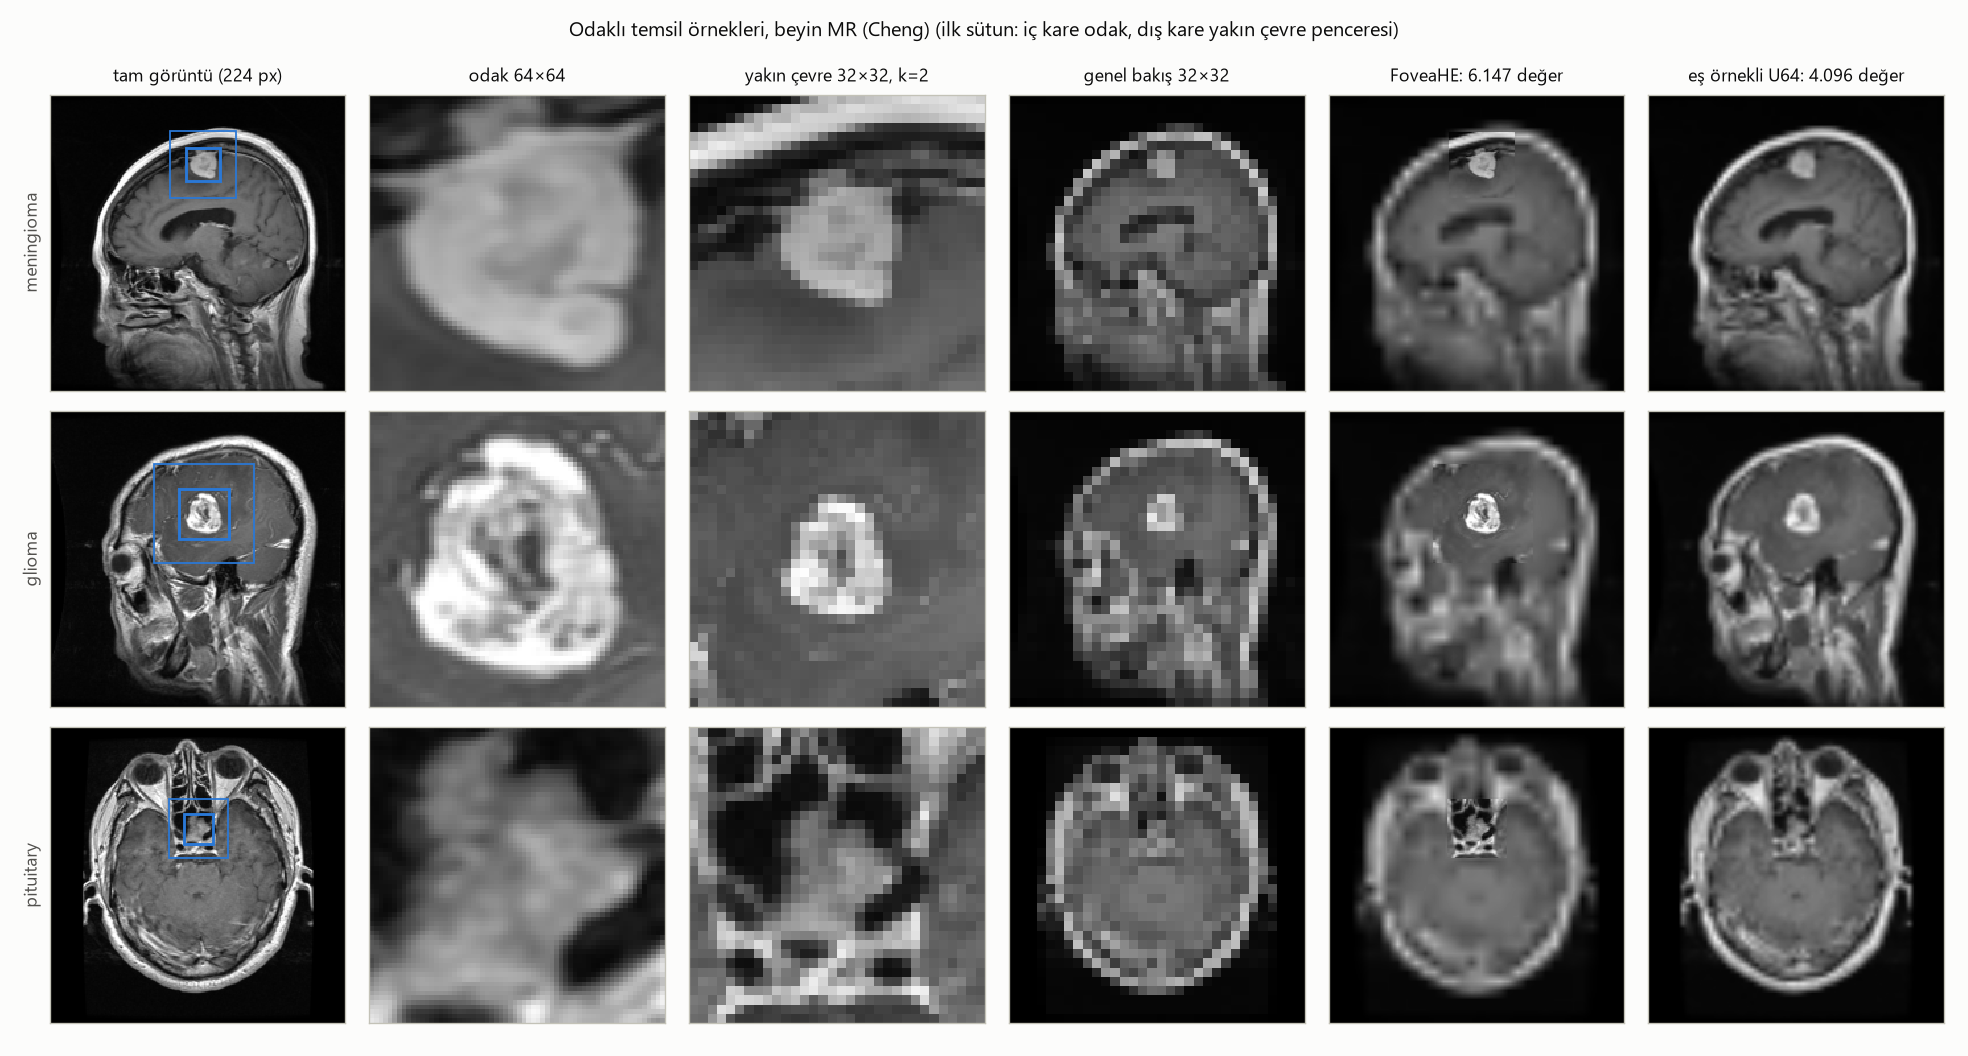
\includegraphics[width=\textwidth,keepaspectratio=true]{./fig/cozum_temsil_ornek_brain}
 \caption{Beyin MR verisinde odaklı temsil örnekleri (satırlar: meningiom, gliom, hipofiz). Sütunlar soldan sağa: pencerelerle tam görüntü (iç kare odak, dış kare yakın çevre penceresi), $64 \times 64$ odak, $32 \times 32$ yakın çevre, $32 \times 32$ genel bakış, bu katmanlardan geri çizilen $224 \times 224$ görüntü ve karşılaştırma için eş örnekli küçültme (U64). Örnekteki yakın çevre katmanı ana yapılandırmalarda kullanılmamıştır.}
 \label{fig:temsil}
\end{figure}

\textbf{Referans temsiller.} Odaklamanın katkısını ayırmak için iki referans kullanılmıştır. \emph{Eş örnekli küçültme} (U$G$), tüm görüntünün yalnızca $G \times G$ örneğidir ve aynı değer bütçesinde odaksız şifrelemeyi temsil eder; örneğin U64 $4.096$ değerdir. \emph{ROI penceresi referansı} ise yalnızca bilgi üst sınırı deneyinde, görüntüye pencerenin konumunu gösteren ek bir kanal ekler. Böylece odaklı temsilin kazancının ROI konum bilgisinden mi, yoksa çözünürlüğün odağa verilmesinden mi geldiği ayrılabilir.

\subsection{Bilgi üst sınırı deneyi}\label{sec:fov:info}

Temsilin teşhis bilgisini koruyup korumadığı, şifreli çalıştırılamayacak kadar güçlü bir modelle ölçülmüştür. Odaklı temsil $224 \times 224$ boyutlu bir görüntüye geri çizilir: her piksel, onu kapsayan en ince katmandan bilineer olarak doldurulur. Bu görüntülerle Saldırı B'deki ResNet-18 eğitim düzeni aynen uygulanmış (beyin MR verisinde 5 kat ve katta 12 dönem, göğüs röntgeninde resmi bölmeler ve 5 dönem) ve sonuç tam görüntüyle eğitilen modelle karşılaştırılmıştır. Beyin MR verisinde 28, göğüs röntgeninde 31 yapılandırmadan oluşan bir ızgara tek tohumla taranmış; seçilen yapılandırmalar ve referanslar 5 tohumla tekrarlanmıştır.

\subsection{Şifreli çalışabilen modellerin eğitimi}\label{sec:fov:models}

Model D, D2 ve C (Bölüm \ref{sec:hemodels}), hem odaklı temsillerde hem de özgün çözünürlükteki tam görüntüde aynı düzenle eğitilmiştir. Tam görüntü üzerindeki Model D, $\Pi_{\mathrm{ROI}}$ protokolünün hesaplama yapısıyla aynıdır. Seçici şifreleme model çıktısını değiştirmediği için bu modelin başarısı $\Pi_{\mathrm{ROI}}$'nin teşhis başarısını temsil eder.

Karşılaştırmanın adil olması için her temsil kendi en iyi ayarını almıştır. AdamW \cite{loshchilov2019adamw} ile ağırlık azaltma $\{10^{-4}, 10^{-2}, 1\}$ kümesinden doğrulama kaybına göre seçilmiştir. En iyi değer üst sınırdaysa arama 10'ar kat genişletilerek $100$'e kadar sürdürülmüş, $100$'e dayanıldığında öğrenme oranı 10 kat düşürülüp $\{100, 1000\}$ değerleri de denenmiştir. Eğitim en çok 200 dönem sürmüş ve doğrulama kaybı 10 dönem boyunca iyileşmediğinde durdurulmuştur. Beyin MR verisinde her test katı için bir sonraki kat doğrulama kümesi olarak, göğüs röntgeninde resmi doğrulama bölmesi kullanılmıştır. Ağırlıklar eğitimden sonra 64 bitlik kayan noktalı sayılara aktarılmış ve aktarılan ağırlıkların eğitilmiş modelle aynı çıktıyı verdiği doğrulanmıştır.

\subsection{Şifreli çıkarım ve maliyet ölçümü}\label{sec:fov:cost}

Şifreli çıkarım TenSEAL ile, $\Pi_{\mathrm{ROI}}$ yeniden üretimindeki CKKS parametreleriyle gerçekleştirilmiştir. Model D ve D2'de şifreli vektörün açık ağırlıklarla iç çarpımları hesaplanmış, Model C'de evrişim pencereleri şifreli metin başına en fazla $8.192$ değerlik parçalar hâlinde matris çarpımıyla işlenmiştir. Şifreli ve şifresiz çıkarımın aynı sonucu verdiği, iki veri kümesinde test bölmesinden sınıf dengeli seçilen 120 görüntüde en büyük logit farkı, tahmin uyumu ve AUC farkıyla ölçülmüştür.

Maliyet, bilgisayarda başka iş çalışmıyorken istemci ön işleme, şifreleme, sunucu hesaplaması ve çözme süreleri ile istemciden sunucuya ve sunucudan istemciye giden veri boyutu olarak ayrı ayrı ölçülmüş ve 3 tekrarın ortalaması alınmıştır. Aynı kod ve aynı ölçüm düzeniyle her model sınıfı için tam görüntünün tam şifrelenmesi ve göğüs röntgeninde gizlilik şartlı $\Pi_{\mathrm{ROI}}$ (\%98 şifreli alan) da ölçülmüştür. Hız kazancı, aynı model sınıfında tam şifreleme toplam süresinin FoveaHE toplam süresine oranı olarak tanımlanmıştır.

\subsection{Sızıntı denetimi}\label{sec:fov:leakage}

FoveaHE'de sunucu açık piksel görmediği için bağlam saldırısı uygulanamaz. Bu nedenle sunucunun görebildiği her bilgi bir saldırganın öznitelikleri olarak kullanılmıştır: şifreli metin sayısı, slot sayısı ve yükleme boyutu (paket meta verisi) ile sunucu hesaplama süresi ve yanıt boyutu (yan kanal). Sınıflandırıcı Saldırı A'daki histogram tabanlı gradyan artırmadır ve 5 tohumla çalıştırılmıştır. Bilgisiz özniteliklerde havuzlanmış kat dışı AUC şans düzeyinden sapabildiğinden, değerlendirmede sınıf dengeli katlar (beyin MR verisinde hasta bazlı) ve kat ortalamalı AUC kullanılmıştır. Saldırganın şans düzeyinden ayırt edilip edilemeyeceği 100 etiket permütasyonuyla sınanmış; gerçek AUC boş dağılımın \%95'lik sınırıyla karşılaştırılmış ve $p$ değeri hesaplanmıştır \cite{ojala2010permutation}.

Denetimin sızıntıyı yakalayabildiğini göstermek için aynı örneklemde $\Pi_{\mathrm{ROI}}$'nin paket meta verisi (ROI şifreli metin sayısı ve yükleme boyutu) pozitif kontrol olarak aynı yöntemle değerlendirilmiştir. Paket meta verisi beyin MR verisinin tamamında ve göğüs röntgeninde sınıf başına 1.000 görüntüde, yan kanal ise sınıf başına 150 görüntüde gerçek şifreli çalıştırmayla ölçülmüştür.

\subsection{Rakip yaklaşımlar}\label{sec:fov:rivals}

\textbf{Şifreli özet.} HETAL \cite{lee2023hetal} tarzında, istemci görüntünün $224 \times 224$ boyutlu kopyasını ImageNet \cite{deng2009imagenet} üzerinde eğitilmiş ve dondurulmuş ResNet-18 \cite{he2016resnet} ile 512 boyutlu bir özete dönüştürür ve özeti şifreler. Sunucu özet üzerinde Model D veya D2'yi şifreli çalıştırır. Eğitim, bölmeler, ayar protokolü, şifreli çıkarım kodu ve CKKS parametreleri FoveaHE ile aynıdır. Ana satırlar 5 tohumla tekrarlanmış, istemcideki ön işleme süresi (görüntü okuma, küçültme ve ResNet-18 ileri geçişi) işlemcide ölçülmüştür.

\textbf{Bozuk bağlam.} Bi-CryptoNets \cite{yuan2024bicryptonets} tarzında, ROI şifreli kalırken açık bağlamın gürültü eklenerek veya bulanıklaştırılarak korunmasının sızıntıyı giderip gidermediği sınanmıştır. Bağlama her görüntü için sabit Gauss gürültüsü ($[0, 1]$ aralığındaki piksel değerleri için $\sigma \in \{0.05, 0.1, 0.2, 0.4\}$) eklenmiş veya ROI hesaba katılmadan normalize edilen Gauss bulanıklığı ($\sigma \in \{2, 4, 8\}$ piksel) uygulanmıştır. Saldırgan Saldırı B'deki gibi eğitilmiş ve aynı bozulmayı eğitimde görerek ona uyum sağlamıştır. Bozulmanın faydaya etkisi, ROI'nin temiz ve bağlamın bozuk olduğu görüşle ölçülmüştür.

\subsection{Bütçe duyarlı odak ve harici derlemede genelleme}\label{sec:fov:bonus}

\textbf{Bütçe duyarlı odak.} Sabit bir şifreli değer bütçesinde çözünürlüğün odak ile genel bakış arasında nasıl paylaştırılması gerektiği incelenmiştir. $B \in \{1.024, 2.048, 4.096, 8.192\}$ bütçeleri ve $s \in \{0, 0.25, 0.5, 0.75, 1\}$ odak payları için $F = \lfloor \sqrt{sB} \rfloor$ ve $G = \lfloor \sqrt{B - F^2 - 3} \rfloor$ alınmıştır; $s = 0$ eş örnekli küçültmeye, $s = 1$ yalnız odağa karşılık gelir. Her yapılandırma Model C ve D ile, Bölüm \ref{sec:fov:models}'teki düzenle ve tek tohumla değerlendirilmiştir.

\textbf{Harici derlemede genelleme.} COVID-QU-Ex ile eğitilen modellerin başka bir derlemeden gelen görüntülerde başarısını koruyup korumadığı, Kaggle kümesinde COVID-QU-Ex içinde karşılığı bulunmayan 1.767 görüntüde (1.157 pnömoni, 340 normal ve 270 COVID-19) sınanmıştır. Görüntüler COVID-QU-Ex gibi $256 \times 256$ boyutuna indirilmiş, ROI olarak Bölüm \ref{sec:transfer}'daki U-Net akciğer maskeleri kullanılmış ve odaklı temsil aynı işlemle çıkarılmıştır. Kaggle sınıfları COVID-QU-Ex sınıflarına eşlenmiş (pnömoni, COVID dışı enfeksiyon sınıfına), modeller 5 tohumun kayıtlı ağırlıklarıyla ve yeniden eğitilmeden uygulanmıştır. Şifreli özet de aynı görüntülerde değerlendirilmiştir.

\subsection{Başarı ölçütleri}\label{sec:fov:criteria}

Sonuçlara göre hedef kaydırılmaması için FoveaHE'nin başarı ölçütleri deneylerden önce belirlenmiş ve sonradan değiştirilmemiştir (Çizelge \ref{tbl:olcutler}). Ana yapılandırmalarda doğruluk deneyleri 5 tohumla tekrarlanmış, güven aralıkları önyüklemeyle (beyin MR verisinde hasta düzeyinde) hesaplanmıştır.

\begin{table*}[h!]
{\setlength{\tabcolsep}{5pt}
\caption{FoveaHE için deneylerden önce belirlenen başarı ölçütleri.}
\begin{center}
\vspace{-6mm}
{\small
\begin{tabular}{lp{9cm}c}
\hline\hline
Ölçüt & Tanım & Eşik \\
\hline
Bilgi kaybı & Tam görüntü ile odaklı temsilin ResNet-18 AUC farkı & $\leq 0.02$ \\
Model kaybı & Aynı model sınıfında tam görüntü ile odaklı temsilin AUC farkı & $\leq 0.03$ \\
Şifreli doğruluk & Şifreli ve şifresiz çıkarımın AUC farkı & $\leq 0.005$ \\
Sızıntı & Sunucunun gördüğü bilgilerle saldırgan AUC değeri & $\leq 0.55$ \\
Hız & Tam şifrelemeye göre toplam süre oranı & $\geq 5$ \\
\hline
\end{tabular}}
\vspace{-6mm}
\end{center}
\label{tbl:olcutler}}
\end{table*}

\section{Yeniden Üretilebilirlik}\label{sec:repro}

Tüm deneyler \texttt{roi-leakage} kod deposunda, proje kökünden tek komutla çalıştırılabilen betikler olarak düzenlenmiş ve git sürüm kontrolüyle kaydedilmiştir. Önerilen yöntem aynı depoda ayrı bir paket olarak uygulanmıştır. Uzun süren çözüm deneyleri, ilerleme yüzdesini ve tahmini bitiş zamanını gösteren ve yarıda kesildiğinde tamamlanmış sonuçları atlayarak kaldığı yerden devam eden bir iş kuyruğuyla çalıştırılmıştır. Deneyler Intel Core i7-10870H işlemci, 16 GB bellek ve 8 GB belleğe sahip NVIDIA GeForce RTX 2070 dizüstü ekran kartından oluşan bir bilgisayarda yapılmıştır. Yazılım ortamı Python 3.13, PyTorch 2.14 (CUDA 12.6), TenSEAL 0.3.16 ve scikit-learn 1.9.1'dir. Rastgele tohumlar sabitlenmiş; ana saldırı görüşleri ve çözümün ana yapılandırmaları 5 farklı tohumla tekrarlanmıştır.
